\documentclass{university}

\subject{تمرین هفتم بخش اول}
\professor{دکتر رهبان}
\student{پارسا محمدیان}

\begin{document}

\setupdocument

\section{}

برای مدل کردن مسئله با 
\lr{Markov Decision Process} 
باید موارد زیر را مشخص کنیم:

\begin{latin}
\begin{itemize}
    \item States
    \item Actions
    \item Transition Function
    \item Reward Function
\end{itemize}
\end{latin}

از آنجایی که نقشه بازی متقارن است، خانه‌ای که روح در آن قراردارد را در 
\lr{States} 
در نظر نمی‌گیریم و در هر حالت صفحه، آن را به نحوی دوران می‌دهیم تا شبیه به شکل 
\ref{fig:states} 
شود. مانطور که در شکل مشخص است، خانه‌ها را شماره گذاری کرده‌ایم و منظورمان از حالت 
\lr{$x$} 
بودن پکمن در خانه 
\lr{$x$} 
است. 

\begin{figure}[htbp]
    \centering
    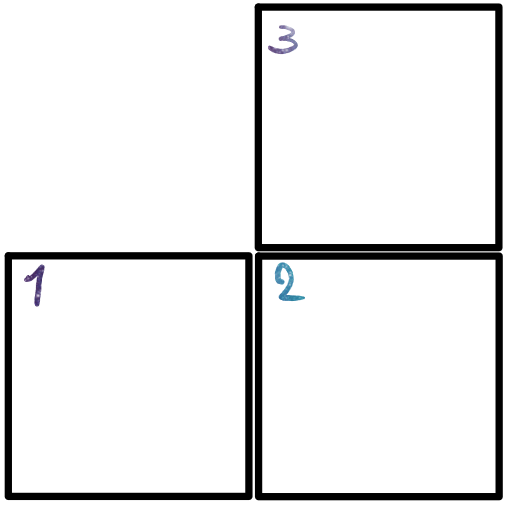
\includegraphics[width=0.6\textwidth]{assets/states.png}
    \caption{\lr{States}}
    \label{fig:states}
\end{figure}

در هر یک از حالت‌ها 
\lr{Actions} 
به صورت بالا پایین چپ راست 
(\lr{$u, d, l, r$})
است. که با توجه به موقعیت برخی از آن‌های مجاز هستند. در حالت 1 بالا رفتن و در حالت 3 چپ رفتن ممنوع است.
\lr{Transition Probabilities} 
به صورت زیر است. 

\begin{gather*}
    T(1, d, 1) = 1 \\
    T(1, l, 1) = 1 \\
    T(1, r, 1) = 0.1 \\
    T(1, r, 2) = 0.9 \\
    T(2, u, 2) = 0.1 \\
    T(2, u, 3) = 0.9 \\
    T(2, d, 2) = 1 \\
    T(2, l, 2) = 0.1 \\
    T(2, l, 1) = 0.9 \\
    T(2, r, 2) = 1 \\
    T(3, u, 3) = 1 \\
    T(3, d, 3) = 0.1 \\
    T(3, d, 2) = 0.9 \\
    T(3, r, 3) = 1
\end{gather*}

\textbf{احتمالاتی که ننوشتم صفر هستند. }

از آنجایی که هدف زنده ماندن است،  
\lr{Reward} 
رفتن به (یا ماندن در) خانه 2 بیشتر از بقیه است. برای مثال این حالت 
\lr{Reward} 
برابر 2 دارد و 
\lr{Reward} 
بقیه حالات 1 است. 

\subsection{}

می‌دانیم سیاست
\lr{Action} 
متناسب با هر 
\lr{State} 
را برای ما مشخص می‌کند. روشی ارائه می‌کنیم که بهترین سیاست را تولید کند. و نتیجه می‌گیریم بهترین سیاست وجود دارد.
 
\lr{$\Pi$} 
را مجموعه تمام سیاست‌های ممکن در نظر می‌گیریم. بدیهتا این مجموعه متناهی است زیرا 
\lr{Actions} 
متناهی است. مشخصا به ازای هر 
\lr{$s \in S$} 
سیاستی وجود دارد که 
\lr{$V(s)$} 
بزرگتر یا مساوی بقیه سیاست‌ها باشد. این 
\lr{Action} 
را در سیاست بهینه‌ای که در حال ساخت آن هستیم به ازای 
\lr{$s$} 
دخیره می‌کنیم. 

در آخر برای این که نشان دهیم سیاست بدست آمده از هر سیاستی بزرگتر است، از برهان خلف استفاده می‌کنیم. فرض می‌کنیم سیاست بزرگتری وجود دارد. 
پس به ازای یک 
\lr{$s \in S$} 
تابع 
\lr{$V(s)$} 
این سیاست بزرگتر است. چون ما اکشن متناظر با بزرگترین 
\lr{$V(s)$} 
را انتخاب کرده‌ایم، به تناقض می‌رسیم. 

\subsection{}

کاملا مشابه حالت قبل اثبات می‌شود.

\end{document}